\documentclass{report}
\usepackage[utf8]{inputenc}
\usepackage[T2A]{fontenc}
\usepackage[russian]{babel}
\usepackage{graphicx}
\usepackage{amsmath}
\usepackage{amsfonts}
\usepackage{amssymb}
\usepackage{bm}

\usepackage{mathtools}
\newcommand\iid{\stackrel{\mathclap{\normalfont\mbox{iid}}}{\sim}}

\setcounter{chapter}{1}


\title{Введение в Бутстреп}
% \author{st013309}
\date{2021}

\begin{document}

\maketitle
\begin{center}
	\textbf{Глава 9}
\end{center}
\textbf{Регрессионные модели}\\
\textbf{9.1 Введение}\\
Регрессионные модели являются одними из самых полезных и наиболее часто используемых статистических методов. Они предлагают относительно простой анализ сложных ситуаций, когда мы пытаемся отсортировать влияние многих возможных объясняющих переменных на зависимую переменную. В главе 7 мы используем алгоритм одновыборочного бутстрепа, алгоритм для анализа точности регрессионного анализа данных холостирамина из таблицы 7.4. Здесь мы более критически смотрим на задачу регрессии. Рассмотрен общий бутстреп алгоритм, показанный на рис. 8.3, что приводит к несколько иному бутстреп анализу для задач регрессии.\\
\textbf{9.2 Линейная регрессионная модель}\\
Мы начнем с классической модели линейной регрессии, или линейной модели, восходящей к Лежандру и Гауссу в начале 19 века. Набор данных $\textbf{x}$ для модели линейной регрессии состоит из $n$ точек $\textbf{x}_1, \textbf{x}_2, \cdots, \textbf{x}_n$, где каждый $\textbf{x}_i$ сам по себе является парой, скажем
$$\textbf{x}_i = (\textbf{c}_i, y_i). \eqno(9.1)$$
Здесь $\textbf{c}_i$ --- это $1 \times p$ вектор $\textbf{c}_i = (c_{il}, c_{i2}, \cdots, c_{ip})$, называемый \textit{вектором признаков} или \textit{предиктором}, а $y_i$ --- действительное число, называемое \textit{ответом}.

Пусть $\mu_i$ указывает условное ожидание $i$-го ответа $y_i$ с учетом предиктора $\textbf{c}_i$,
$$\mu_i = \text{E}(y_i|\textbf{c}_i) \quad (i = 1,2, \cdots, n). \eqno(9.2)$$
Ключевое предположение в линейной модели состоит в том, что $\mu_i$ представляет собой линейную комбинацию компонентов предиктора $\textbf{c}_i$,
$$\mu_i = \textbf{c}_i \bm{\beta} = \sum\limits_{j=1}^{p} c_{ij} \beta_j. \eqno(9.3)$$
\textit{Вектор параметров}, или \textit{параметр регрессии}, $\bm{\beta} = (\beta_1, \beta_2, \cdots, \beta_p)^\text{T}$ неизвестен, обычная цель регрессионного анализа состоит в том, чтобы вывести $\bm{\beta}$ из наблюдаемых данных $\textbf{x} = (\textbf{x}_1, \textbf{x}_2, \cdots, \textbf{x}_n)$. В квадратичной регрессии (7.20) для данных холостирамина ответ $y_i$ --- это улучшение для $i$-го человека, признак $\textbf{c}_i$ --- это вектор $(1, z_i, z_i^2)$ и $\bm{\beta} = (\beta_0, \beta_1, \beta_2)^\text{T}$. \underline{Примечание}: «Линейность» в линейной регрессии относится к линейной форме математического ожидания (9.3). Нет никакого противоречия в том, что линейная модель (7.20) является квадратичной функцией $z$.

Вероятностная структура линейной модели обычно выражается как
$$y_i = \textbf{c}_i \bm{\beta} + \varepsilon_i \quad \text{для} \quad i = 1,2,\cdots,n. \eqno(9.4)$$
Предполагается, что ошибка $\varepsilon_i$ в (9.4) является случайной выборкой из неизвестного \textit{распределения ошибок} $F$ с математическим ожиданием $0$,\\

\noindent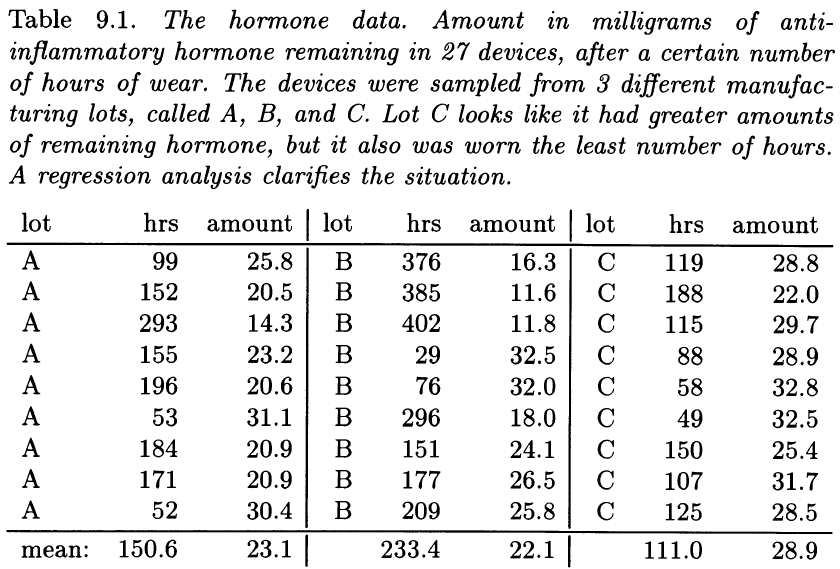
\includegraphics[width=12cm]{tab91}

$$F \to (\varepsilon_1, \varepsilon_2, \cdots, \varepsilon_n) = \bm{\varepsilon} \quad [\text{E}_F(\bm{\varepsilon})=0]. \eqno(9.5)$$

Заметим, что (9.4), (9.5) влекут

\begin{tabular}{c c l}
	$\text{E}(y_i|\textbf{c}_i)$ & = & $\text{E}(\textbf{c}_i \bm{\beta}+\varepsilon_i|\textbf{c}_i) = \text{E}(\textbf{c}_i \bm{\beta}|\textbf{c}_i) + \text{E}(\varepsilon_i|\textbf{c}_i)$\\
	& = & $\textbf{c}_i \bm{\beta},$
\end{tabular} $$\eqno(9.6)$$
что является предположением о линейности (9.3). Здесь мы использовали тот факт, что условное ожидание $\text{E}(\varepsilon_i|\textbf{c}_i)$ совпадает с безусловным ожиданием $\text{E}(\varepsilon_i) = 0$, поскольку $\varepsilon_i$ выбираются независимо от $\textbf{c}_i$.

Мы хотим оценить вектор параметра регрессии $\bm{\beta}$ из наблюдаемых данных $(\textbf{c}_1, y_1), (\textbf{c}_2, y_2), \cdots, (\textbf{c}_n, y_n)$. Пробное значение $\bm{\beta}$, скажем $\textbf{b}$, дает \textit{остаточную квадратичную ошибку}
$$\text{RSE}(\textbf{b}) = \sum\limits_{i=1}^{n} (y_i - \textbf{c}_i \textbf{b})^2, \eqno(9.7)$$
как в уравнении (7.21). Оценка \textit{методом наименьших квадратов} $\bm{\beta}$ --- это значение $\hat{\bm{\beta}}$ из $\textbf{b}$, которое минимизирует $\text{RSE}(\textbf{b})$,
$$\text{RSE}(\hat{\bm{\beta}}) = \min_{\textbf{b}} [\text{RSE(\textbf{b})}]. \eqno(9.8)$$		
Пусть $\textbf{C}$ --- матрица размера $n \times p$ с $i$-й строкой $\textbf{c}_i$ (design matrix), а \textbf{y} --- вектор $(y_1, y_2, \cdots, y_n)^\text{T}$. Тогда оценка методом наименьших квадратов является решением следующего уравнения
$$\textbf{C}^\text{T} \textbf{C} \hat{\bm{\beta}} = \textbf{C}^\text{T} \textbf{y} \eqno(9.9)$$
и задается формулой
$$\hat{\bm{\beta}} = (\textbf{C}^\text{T} \textbf{C})^{-1} \textbf{C}^\text{T} \textbf{y}. \eqno(9.10)$$\\
\textbf{9.3 Пример: данные по гормонам}\\
В таблице 9.1 показан небольшой набор данных, который является подходящим для регрессионного анализа. Медицинское устройство для непрерывной доставки противовоспалительного гормона было протестировано на $27$ пациентах. Переменная ответа $y_i$ --- это количество гормона, оставшееся в устройстве после ношения,
$$y_i = \text{ оставшееся количество гормона в устройстве} i, \; i = 1, 2, \cdots, 27.$$
Есть две переменные--предикторы,
$$z_i = \text{ количество часов ношения i-го устройства}$$
и
$$L_i = \text{ производственная партия устройства i}.$$
Тестируемые устройства были случайным образом выбраны из трех различных производственных партий, названных $A$, $B$ и $C$.

Левая часть рисунка 9.1 представляет собой диаграмму рассеяния 27 точек $(z_i, y_i) = (\text{часы}_i, \text{число}_i)$ с символом $L_i$, используемым в качестве графического сивола. Мы видим, что более длительное время ношения приводит к меньшему количеству оставшегося гормона, как и следовало ожидать. Мы можем количественно оценить это наблюдение с помощью регрессионного анализа.

Рассмотрим модель, в которой математическое ожидание $y$ является линейной функцией $z$,

$$\mu_i = \text{E}(y_i|z_i) = \beta_0 + \beta_1 z_i \quad i = 1,2, \cdots, 27. \eqno(9.11)$$
Эта модель игнорирует $L_i$: он имеет форму (9.3) с векторами признаков размерности $p = 2$,
$$\textbf{c}_i = (1, z_i). \eqno(9.12)$$
Вектор неизвестных параметров $\bm{\beta}$ был помечен $(\beta_0, \beta_1)$ вместо $\beta_1, \beta_2$, так что индексы соответствуют степеням $z$, как в (7.20). Нормальные уравнения (9.10) дают оценку наименьших квадратов
$$\hat{\bm{\beta}} = (34.17, -0.0574)^\text{T}. \eqno(9.13)$$
Линия регрессии, оцененная методом наименьших квадратов
$$\hat{\mu}_i = \textbf{c}_i \hat{\bm{\beta}} = \hat{\beta}_0 + \hat{\beta}_1 z_i \eqno(9.14)$$
изображена на правой части рисунка 9.1. Среди всех возможных линий, которые можно было нарисовать, эта линия минимизирует сумму квадратов $27$ вертикальных расстояний от точек до линии.
	
\noindent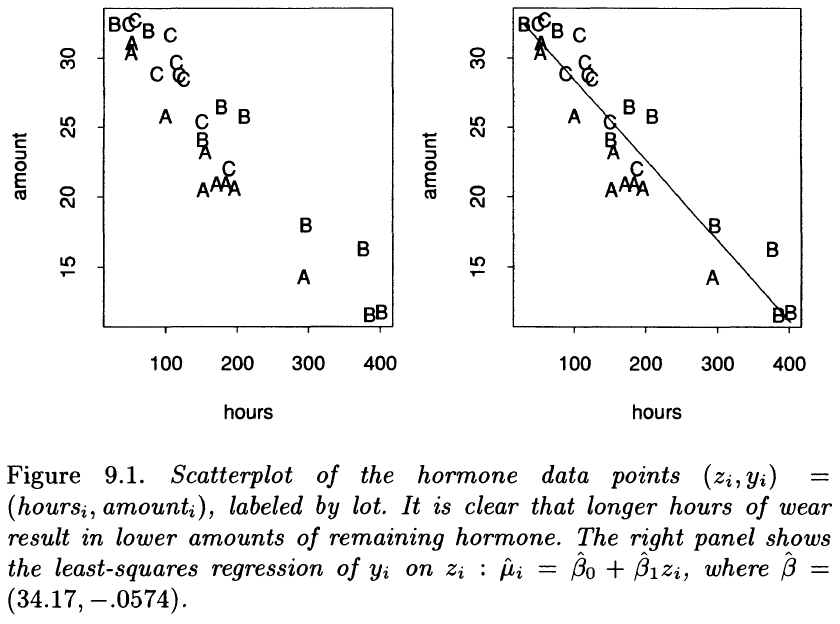
\includegraphics[width=12cm]{fig91}
	
Насколько точен оценочный вектор параметров $\hat{\bm{\beta}}$? Ответ дает чрезвычайно полезная формула, также восходящая к Лежандру и Гауссу. Пусть $\textbf{G}$ --- матрица скалярных произведений $p \times p$,
$$\textbf{G} = \textbf{C}^\text{T}\textbf{C}, \eqno(9.15)$$

\noindent матрица с элементом $g_{hj} = \sum\limits_{i=1}^{n} c_{ih} c_{ij}$ в строке $h$, столбце $j$. Пусть $\sigma^2_F$ будет дисперсией ошибок в модели (9.4),

$$\sigma^2_F = \text{var}_F(\varepsilon). \eqno(9.16)$$

Тогда стандартная ошибка $j$-го компонента $\hat{\bm{\beta}}$, квадратного корня из его дисперсии, равна
$$\text{se}(\hat{\beta}_j) = \sigma_F \sqrt{G^{jj}} \eqno(9.17)$$
где $G^{jj}$ --- $j$-й диагональный элемент обратной матрицы $\textbf{G}^{-1}$.

Последняя формула является обобщением формулы (5.4) для стандартной ошибки выборочного среднего, $\text{se}_F(\bar{x}) = \sigma_F / \sqrt{n}$, см. задачу 9.1. На практике $\sigma_F$ оценивается по формуле, аналогичной (5.11),
$$\hat{\sigma}_F = \{ \sum\limits_{i=1}^{n} (y_i - \textbf{c}_i \hat{\bm{\beta}})^2 / n \}^{1/2} = \{ \text{RSE}(\hat{\bm{\beta}})/n \}^{1/2} \eqno(9.18)$$
или версией $\hat{\sigma}_F$ с корректированным смещением,

\noindent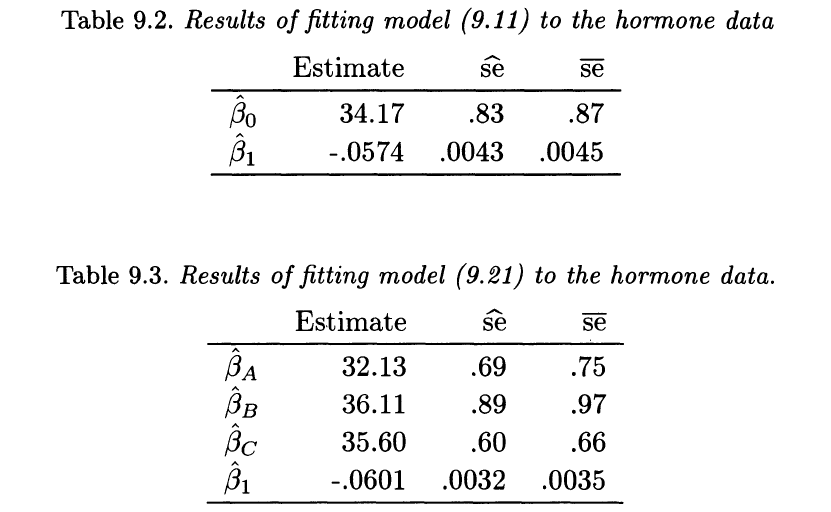
\includegraphics[width=12cm]{tab92tab93}

$$\bar{\sigma}_F = \{ \text{RSE}(\hat{\bm{\beta}})/(n-p) \}^{1/2}. \eqno(9.19)$$
Соответствующие оценочные стандартные ошибки для компонентов $\hat{\bm{\beta}}$ равны

$$\hat{\text{se}}(\hat{\beta}_j) = \hat{\sigma}_F \sqrt{G^{jj}} \text{  или  } \bar{\text{se}} (\hat{\beta}_j) = \hat{\sigma}_F \sqrt{G^{jj}}. \eqno(9.20)$$

\noindent Связь между $\hat{\text{se}}(\hat{\beta}_j)$ и $\bar{\text{se}}(\hat{\beta}_j)$ такая же, как между формулами (5.12) и (2.2) для среднего.

Большинство программ для линейной регрессии с библиотеками обычно выдают результат $\bar{\text{se}}(\hat{\beta}_j)$ вместе с оценкой $\hat{\beta}_j$ методом наименьших квадратов. Применение такой программы к модели (9.11) для данных по гормону дает результаты в таблице 9.2.

Глядя на правую часть рисунка 9.1, большинство точек для партии $A$ лежат ниже подобранной линии регрессии, в то время как большинство точек для партий $B$ и $C$ лежат выше этой линии. Это говорит о неточности модели (9.11). Если бы модель была точной, можно было бы ожидать, что примерно половина каждой партии будет лежать выше, а половина ниже установленной линии. Выражаясь обычной терминологией, похоже, что в данных присутствует эффект партии.

В нашу линейную модель легко включить эффект партии. Мы предполагаем, что условное математическое ожидание $y$ при заданных $L$ и $z$ имеет вид
$$\text{E}(y|L,z) = \beta_L + \beta_1 z. \eqno(9.21)$$
Здесь $B_L$ равно одному из трех возможных значений: $\beta_A, \beta_B, \beta_C$, в зависимости от партии устройства. Это похоже на модель (9.11), за исключением того, что (9.21) допускает разные точки пересечения для каждой партии, а не одну точку пересечения $\beta_0$ из (9.11). Анализ модели (9.21) методом наименьших квадратов дал результаты в таблице 9.3.

Обратите внимание, что $\hat{\beta}_A$ на несколько стандартных ошибок меньше чем $\hat{\beta}_B$ и $\hat{\beta}_C$, что указывает на то, что устройства в партии $A$ содержат значительно меньше гормона.\\
\textbf{9.4 Применение бутстрепа}\\
Пока ни один из расчетов не требует бутстрепа. Однако полезно выполнить бутстреп-анализ для модели линейной регрессии. Оказывается, оценки стандартной ошибки бустрепа такие же, как $\hat{\text{se}}(\hat{\beta}_j)$, (9.20). Убедившись, что бутстреп дает разумные ответы в случае, который мы можем проанализировать математически, мы можем продолжить применять бутстреп к более общим моделям регрессии, которые не имеют математического решения: где функция регрессии нелинейна по параметрам $\bm{\beta}$, и где мы используем методы подбора, отличные от метода наименьших квадратов.
	
Вероятностная модель $P \to \textbf{x}$ для линейной регрессии, как описано в (9.4), (9.5), состоит из двух компонентов:
$$P = (\bm{\beta}, F), \eqno(9.22)$$
где $\bm{\beta}$ --- вектор параметров коэффициентов регрессии, а $F$ --- распределение вероятностей ошибок. Общий алгоритм бустрепа на рис. 8.3 требует, чтобы мы оценили $P$. У нас уже есть доступная $\hat{\bm{\beta}}$, оценка методом наименьших квадратов для $\bm{\beta}$. Как мы можем оценить $F$? Если бы $\bm{\beta}$ было известно, мы могли бы вычислить ошибки $\varepsilon_i = y_i - \textbf{c}_i \bm{\beta}$ для $i = 1,2, \cdots, n$ и оценить $F$ по их эмпирическому распределению. Мы не знаем $\bm{\beta}$, но можем использовать $\hat{\bm{\beta}}$ для вычисления аппроксимации ошибок
$$\hat{\varepsilon}_i = y_i - \textbf{c}_i \hat{\bm{\beta}}, \text{  для  } i = 1,2, \cdots, n. \eqno(9.23)$$
($\hat{\varepsilon}_i$ также называют \textit{остатками}.) Очевидная оценка $F$ --- это эмпирическое распределение $\hat{\varepsilon}_i$,
$$\hat{F}: \text{ вероятность } 1/n \text{ для } \hat{\varepsilon}_i \text{ при } i = 1,2, \cdots, n. \eqno(9.24)$$
Обычно $\hat{F}$ будет иметь ожидание $0$, как требуется в (9.5), см. задачу 9.5.
					
Имея в руках $\hat{P} = (\hat{\bm{\beta}}, \hat{F})$, мы знаем, как рассчитать наборы данных бутстрепа для модели линейной регрессии: $\hat{P} \to \textbf{x}^*$ должно означать то же самое, что и $P \to \textbf{x}$, вероятностный механизм (9.4), (9.5), дающий фактический набор данных $\textbf{x}$. Чтобы сгенерировать $\textbf{x}^*$, мы сначала выбираем случайную выборку бустреп ошибок
$$\hat{F} \to (\varepsilon_1^*, \varepsilon_2^*, \cdots, \varepsilon_n^*) = \bm{\varepsilon}^*. \eqno(9.25)$$
Каждый $\varepsilon_i^*$ равен любому из $n$ значений $\hat{\varepsilon}_j$ с вероятностью $1 / n$. Затем бустреп ответы $y_i^*$ генерируются согласно (9.4),
$$y_i^* = \textbf{c}_i \hat{\bm{\beta}} + \varepsilon_i^* \text{  для  } i = 1,2,\cdots,n. \eqno(9.26)$$
Читатель должен убедиться, что (9.24), (9.25), (9.26) то же самое, что (9.4), (9.5), за исключением того, что $\hat{P} = (\hat{\bm{\beta}}, \hat{F})$ заменяет $P = (\bm{\beta}, F)$. Обратите внимание, что $\hat{\bm{\beta}}$ --- фиксированная величина в (9.26), имеющая одинаковые значения для всех $i$.
	
Бутстреп набор данных $\textbf{x}^*$ равен $(\textbf{x}_1^*, \textbf{x}_2^*, \cdots, \textbf{x}_n^*)$, где $\textbf{x}_i^* = (\textbf{c}_i, y_i^*)$. Может показаться странным, что векторы признаков $\textbf{c}_i$ для бутстреп данных такие же, как и для фактических данных. Это происходит потому, что мы рассматриваем $\textbf{c}_i$ как фиксированные величины, а не как случайные. (Во всех наших примерах размер выборки $n$ трактовался одинаково.) Этот момент дополнительно обсуждается ниже.
	
Бустреп оценка $\hat{\bm{\beta}}^*$ методом наименьших квадратов является минимизатором квадратичной остаточной ошибки для бустреп данных,
$$\sum\limits_{i=1}^{n}(y_i^* - \textbf{c}_i \hat{\bm{\beta}}^*)^2 = \min_{\textbf{b}} (y_i^* - \textbf{c}_i \textbf{b})^2. \eqno(9.27)$$
Нормальные уравнения (9.10), примененные к бутстреп данным, дают
$$\hat{\bm{\beta}}^* = (\textbf{C}^\text{T} \textbf{C})^{-1} \textbf{C}^\text{T} \textbf{y}^*. \eqno(9.28)$$

В этом случае нам не нужны симуляции Монте--Карло, чтобы вычислить бутстреп стандартные ошибки для компонентов $\hat{\bm{\beta}}^*$. Несложный расчет дает выражение в явной форме для $\text{se}_{\hat{F}} (\hat{\bm{\beta}}_j^*) = \hat{\text{se}}_{\infty} (\hat{\beta}_j)$, идеальной оценки бутстреп стандартной ошибки:\\

\begin{tabular}{ccl}
	$\text{var}(\hat{\bm{\beta}}^*)$ & = & $(\textbf{C}^\text{T} \textbf{C})^{-1} \textbf{C}^\text{T} \text{var}(\textbf{y}^*) \textbf{C}(\textbf{C}^\text{T} \textbf{C})^{-1}$ \\
	& = & $\hat{\sigma}_F^2 (\textbf{C}^\text{T} \textbf{C})^{-1},$
\end{tabular} $$\eqno(9.29)$$
поскольку $\text{var}(\textbf{y}^*) = \hat{\sigma}^2_F \textbf{I}$, где $\textbf{I}$ --- единичная матрица. Следовательно
$$\hat{\text{se}}_{\infty}(\hat{\beta}_j) = \hat{\sigma}_F \sqrt{G^{jj}}. \eqno(9.30)$$
Другими словами, бутстреп оценка стандартной ошибки для $\hat{\beta}_j$ такая же, как и обычная оценка $\hat{\text{se}}(\hat{\beta}_j)$, (9.20).\\
\textbf{9.5 Бутстреп пары против бутстреп остатков}\\
Читатель, возможно, заметил интересный факт: теперь у нас есть два разных способа бутстреп регрессионной модели. Метод, описанный в главе 7, выбирал пары $\textbf{x}_i = (\textbf{c}_i, y_i)$, так что бутстреп набор данных $\textbf{x}^*$ имел форму
$$\textbf{x}^* = \{ (\textbf{c}_{{i}_1}, y_{{i}_1}), (\textbf{c}_{{i}_2}, y_{{i}_2}), \cdots, (\textbf{c}_{{i}_n}, y_{{i}_n}) \}, \eqno(9.31)$$
для $i_1, i_2, \cdots, i_n$ в случайной выборке целых чисел от $1$ до $n$. Обсуждаемый в этой главе метод (9.24), (9.25), (9.26) можно назвать «бутстрепом остатков». Он создает бутстреп наборы данных в форме
$$\textbf{x}^* = \{ (\textbf{c}_1, \textbf{c}_1 \hat{\bm{\beta}} + \hat{\varepsilon}_{{i}_1}), (\textbf{c}_2, \textbf{c}_2 \hat{\bm{\beta}} + \hat{\varepsilon}_{{i}_2}), \cdots, (\textbf{c}_n, \textbf{c}_n \hat{\bm{\beta}} + \hat{\varepsilon}_{{i}_n}) \}. \eqno(9.32)$$

\noindent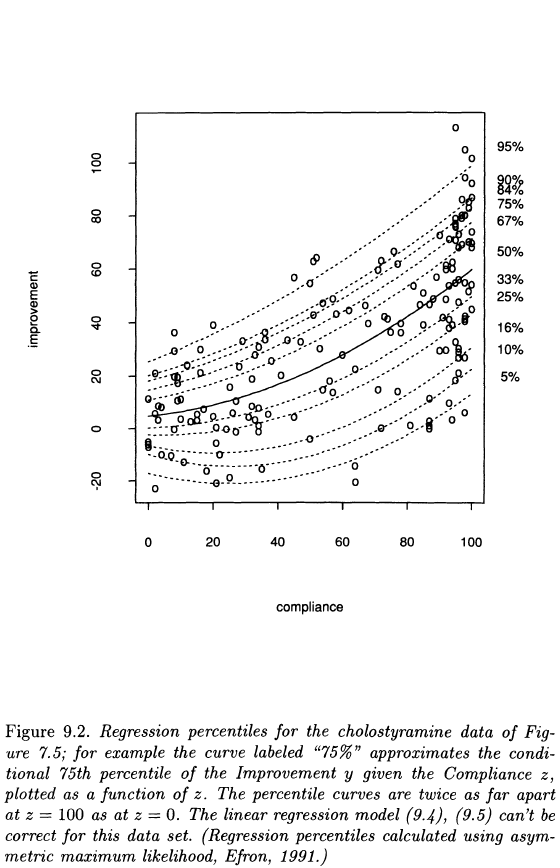
\includegraphics[width=12cm]{fig92}\\

Какой бутстреп метод лучше? Ответ зависит от того, насколько мы доверяем модели линейной регрессии (9.4). Эта модель говорит, что ошибка между $y_i$ и его средним значением $\mu_i = \textbf{c}_i \bm{\beta}$ не зависит от $\textbf{c}_i$; он имеет одинаковое распределение «$F$» независимо от $\textbf{c}_i$. Это сильное предположение, которое может оказаться неверным, даже если модель математического ожидания $\mu_i = \textbf{c}_i \bm{\beta}$ верна. Это не соответствует данным холостирамина на рис. 7.4.

На рисунке 9.2 показаны \textit{процентили регрессии} для данных холостирамина. Например, кривая, обозначенная «$75$\%», аппроксимирует условный $75$-й процентиль улучшения $y$ как функцию соответствия $z$. Вблизи любого заданного значения $z$ около $75$\% нанесенных на график точек лежат ниже кривой. Модель (9.4), (9.5) предсказывает, что эти кривые будут находиться на одинаковом расстоянии друг от друга для всех значений $z$. Вместо этого кривые расходятся по мере увеличения $z$, будучи вдвое дальше друг от друга при $z = 100$, чем при $z = 0$. Другими словами, ошибки $\varepsilon_i$ в (9.4) стремятся быть вдвое больше при $z = 100$, чем при $z = 0$.

Бутстреп пары менее чувствительны к предположениям, чем бутстреп остатки. Стандартная оценка ошибки, полученная с помощью бутстреп пар (9.31), дает разумные ответы, даже если (9.4), (9.5) полностью неверны. Единственное предположение, стоящее за (9.31), состоит в том, что исходные пары $\textbf{x}_i = (\textbf{c}_i, y_i)$ были случайным образом выбраны из некоторого распределения $F$, где $F$ --- распределение на $(p+1)$--мерных векторах $(\textbf{c}, y)$. Даже если (9.4), (9.5) верны, нет ничего плохого в бустреп парах, как показано в (9.31); можно показать, что ответ (9.31) приближается к ответу (9.32) по мере увеличения числа пар $n$. Простая модель для данных гормонов (9.12) была повторно проанализирована бутстреп-парами. $B = 800$ бутстреп репликаций дали
$$\hat{\text{se}}_{800} (\hat{\beta}_0) = 0.77 \quad \hat{\text{se}}_{800}(\hat{\beta}_1) = 0.0045, \eqno(9.33)$$
что не сильно отличается от таблицы 9.2.

Можно привести и обратный аргумент. Модель (9.4), (9.5) не обязательно должна выполняться идеально, чтобы бутстреп остатков, как в (9.32), давал разумные результаты. Более того, различия в распределении ошибок, как и в данных холостирамина, могут быть включены в модель (9.4), (9.5), что приведет к более подходящей версии бутстреп остатков; см. модель (9.42). Возможно, наиболее важным моментом здесь является то, что бутстреп не является однозначно определенной концепцией. Рисунок 8.3 может быть реализован по-разному для одной и той же задачи, в зависимости от того, как интерпретируется вероятностная модель $P \to \textbf{x}$.

Когда мы осуществляем бустреп остатков, бутстреп наборы данных $\textbf{x}^* = \{(\textbf{c}_1, y_1^*), (\textbf{c}_2, y_2^*), \cdots, (\textbf{c}_n, y_n^*)\}$ имеют вектора признаков $\textbf{c}_1, \textbf{c}_2, \cdots, \textbf{c}_n$ в точности такие же, как и для фактического набора данных $\textbf{x}$. Это кажется неестественным для данных по гормонам, где $\textbf{c}_i$ включает $z_i$, затраченное количество часов, которое является такой же случайной величиной, как и переменная ответа $y_i$, оставшееся количество гормона.

Даже когда признаки генерируются случайным образом, есть причины проводить анализ так, как если бы они были фиксированными. Коэффициенты регрессии имеют большую стандартную ошибку, когда признаки имеют меньшее стандартное отклонение. Рассматривая признаки как фиксированные константы, мы получаем стандартную ошибку, которая отражает точность, связанную с выборкой фактически наблюдаемых признаков. Однако, как показывает (9.33), разница между $\textbf{c}_i$ фиксированной и $\textbf{c}_i$ случайной обычно не сильно влияет на оценку стандартной ошибки.\\
\textbf{9.6 Пример: данные о выживаемости клеток}\\
Бывают ситуации в регрессии, когда признаки более естественно считать фиксированными, а не случайными. Данные по выживаемости клеток в таблице 9.4 показывают такую ситуацию. Радиолог провел эксперимент с 14 бактериальными пластинами. Пластинки подвергали воздействию различных доз радиации и измеряли долю выживших клеток. Как и следовало ожидать, более высокие дозы приводят к меньшей выживаемости. Знак вопроса после ответа на пластине $13$ отражает некоторую неуверенность в этом результате, выраженную исследователем.

Исследователя интересовал регрессионный анализ с переменной--предиктором.
$$\text{доза}_i = z_i \quad i = 1,2, \cdots, 14 \eqno(34)$$
и переменная ответа
$$\log \text{(пропорция выживания)}_i = y_i \quad i=1,2,\cdots 14. \eqno(9.35)$$
Были доступны две различные теоретические модели радиационного поражения, одна из которых предсказывала линейную регрессию,
$$\mu_i = \text{E}(y_i|z_i) = \beta_1 z_i, \eqno(9.36)$$
и другая квадратичная регрессия,
$$\mu_i = \text{E}(y_i|z_i) = \beta_1 z_i + \beta_2 z_i^2. \eqno(9.37)$$
В (9.36) или (9.37) нет пересекающих членов $\beta_0$, потому что мы знаем, что нулевая доза дает коэффициент выживаемости $1$, $y = \log (1) = 0$.

В таблице 9.5 показаны оценки методом наименьших квадратов $(\hat{\beta}_1, \hat{\beta}_2)$ и их оценочные стандартные ошибки $\bar{\text{se}}(\hat{\beta}_j)$, (9.20). Представлены два анализа методом наименьших квадратов, один с данными для всех $14$ пластин, другой за исключением сомнительной пластины $13$. В обоих анализах оцененный коэффициент квадратичной регрессии $\hat{\beta}_2$ является положительным. Является ли это отличие значимым? Другими словами, можем ли мы заключить, что $\hat{\beta}_2$ останется положительным, если будет исследовано гораздо больше пластин? Отношение $\hat{\beta}_2/\hat{\text{se}}(\hat{\beta}_2)$ помогает ответить на этот вопрос. Отношение составляет $2.46$ для анализа, основанного на всех $14$ пластинах, что обычно считается убедительным доказательством того, что $\hat{\beta}_2$ значительно больше нуля. Если верить этому результату, то квадратичная модель (9.37) сильно предпочтительнее модели (9.36), которая имеет $\beta_2 = 0$.
				
\noindent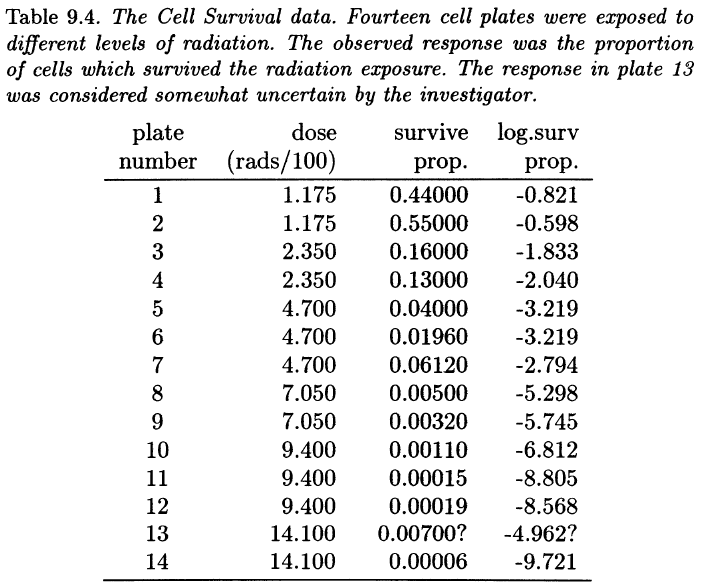
\includegraphics[width=12cm]{tab94}

Однако удаление сомнительной пластины $13$ из анализа снижает $\hat{\beta}_2/\hat{\text{se}}(\hat{\beta}_j)$ только до $0.95$, что является \underline{несущественным} результатом. Вывод заключается не в том, что $\beta_2$ \textit{обязательно} равен нулю, а в том, что он легко может быть равен нулю: если $\beta_2 = 0$, и если $(\beta_2) \dot = 0.0091$, как в строке 2 таблицы 9.5, то это вовсе не удивительно, что значение $\hat{\beta}_2$ такое же большое или больше наблюдаемого значения $0.0086$. У нас нет убедительных доказательств для отказа от линейной модели в пользу квадратичной модели.
							
Статистика --- это наука о сборе информации по крупицам с целью получения высокоинформативных сложных результатов. Статистики настораживаются, когда видят, что одна точка данных, особенно подозрительная, доминирует в ответе на важный вопрос. Действительная критика регрессии по методу наименьших квадратов состоит в том, что одна удаленная точка, такая как пластина $13$, может иметь слишком большое влияние на подобранную кривую регрессии. Это показано на рисунке 9.3, который строит кривую регрессии методом наименьших квадратов как с данными из пластины $13$, так и без них. Мощный эффект точки «?» очевиден. Даже если бы исследователь не подвергал сомнению достоверность пластинки $13$, мы бы предпочли, чтобы наши подогнанные кривые не зависели так сильно от отдельных точек данных.\\

\noindent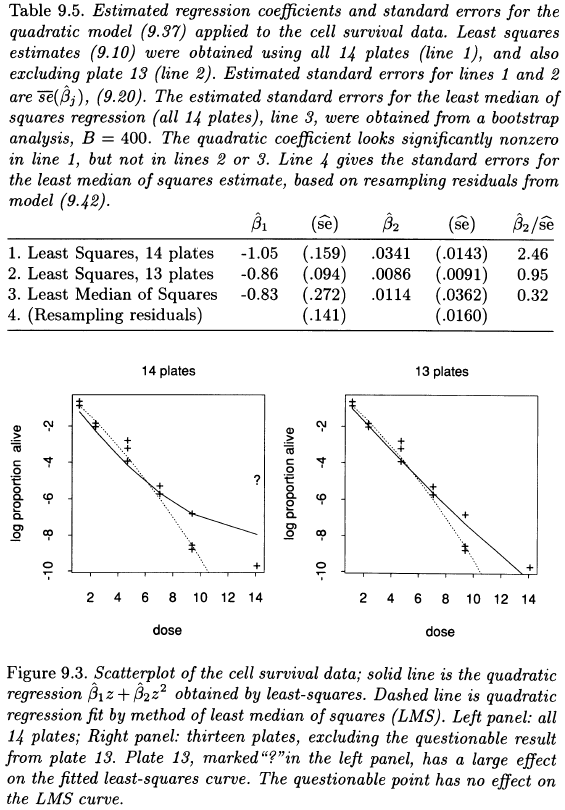
\includegraphics[width=12cm]{tab95fig93}

\newpage

\noindent\textbf{9.7 Наименьшая медиана квадратов}\\
Наименьшая медиана квадратов регрессии, сокращенно $\text{LMS}$, является менее чувствительным методом подбора, чем метод наименьших квадратов. Единственное различие между методом наименьших квадратов и $\text{LMS}$ --- это выбор \underline{критерия соответствия}. Чтобы \underline{motivate} критерий, давайте разделим остаточную квадратичную ошибку (9.7) на размер выборки, получив среднеквадратичные остатки
$$\dfrac{1}{n} \sum\limits_{i=1}^{n} (y_i-\textbf{c}_i \textbf{b})^2. \eqno(9.38)$$

\noindent Минимизация (9.38), очевидно, то же самое, что минимизация (9.7). Средние выборок чувствительны к влияющим значениям, а медианы --- нет. Следовательно, чтобы сделать (9.38) менее чувствительным, мы можем заменить среднее значение на медиану, получив \textit{\underline{медианноквадратичные остатки}}
$$\text{MSE}(\textbf{b}) = \text{медиана}(y_i - \textbf{c}_i \textbf{b})^2. \eqno(9.39)$$
Оценка $\text{LMS}$ $\bm{\beta}$ --- это значение $\hat{\bm{\beta}}$, минимизирующее $\text{MSR(\textbf{b})}$,
$$\text{MSR}(\hat{\bm{\beta}}) = \min_{\textbf{b}} [\text{MSR}(\textbf{b})]. \eqno(9.40)$$

Обратите внимание, что разница между методом наименьших квадратов и $\text{LMS}$ заключается не в выборе модели, которая остается (9.3), а в том, как мы измеряем расхождения между моделью и наблюдаемыми данными. $\text{MSR}(\textbf{b})$ менее чувствителен, чем $\text{RSE}(\textbf{b})$, к удаленным точкам данных. Это можно увидеть на рис. 9.3, где, по-видимому, очень мало различий между квадратичной $\text{LMS}$-аппроксимацией с точкой «?» или без нее. На самом деле разницы нет. Расчетные коэффициенты регрессии равны $(\hat{\beta}_1, \hat{\beta}_2) = (-0.81, 0.0088)$ в обоих случаях.

Можно показать, что \textit{\underline{разбивка}} оценки $\text{LMS}$ составляет примерно $50\%$. \underline{Разбивка} оценщика --- это наименьшая часть данных, которая может \underline{произвольно сильно} повлиять на ее значение. Другими словами, оценщик имеет \underline{разбивку $\alpha$}, если по крайней мере $m = \alpha \cdot n$ точек данных должны быть «плохими», прежде чем он разобьет. Высокая \underline{разбивка} --- это хорошо, при этом $50\%$ --- это наибольшее значение, которое имеет смысл (если $\alpha> 50\%$, неясно, какие из них являются хорошими, а какие плохими). Например, среднее значение выборки имеет \underline{разбивку} $1 / n$, поскольку, изменяя только одно значение данных, мы можем заставить среднее значение выборки принимать любое значение. Медиана выборки имеет \underline{разбивку} $50\%$, что отражает тот факт, что она менее чувствительна к отдельным значениям. Оценщик регрессии методом наименьших квадратов наследует чувствительность среднего и имеет \underline{разбивку} $1 / n$, в то время как оценщик наименьших средних квадратов, как и медиана, имеет \underline{разбивку} примерно $50\%$. Точное определение \underline{разбивки} дано в задаче 9.9.

Насколько точны $\text{LMS}$ оценки $\hat{\beta}_1, \hat{\beta}_2$? Нет четкой формулы, подобной (9.20) для стандартных ошибок $\text{LMS}$. (Нет четкой формулы для самих оценок $\text{LMS}$. Они вычисляются с использованием алгоритма выборки с возвращением: см. задачу 9.8.) Стандартные ошибки в таблице 9.5 были получены методами бутстрепа. Стандартные ошибки в строке 3 основаны на парах повторной выборки, как в разделе 7.3. Бустреп набор данных был создан в форме $\textbf{x}^* = ((\textbf{c}_1^*, y_1^*), (\textbf{c}_2^*, y_2^*), \cdots, (\textbf{c}_n^*, y_n^*))$, как в (9.31), где $\textbf{c}_i = (z_i, z_i^2)$. После генерации $\textbf{x}^*$ была получена репликация бутстрепа $\hat{\bm{\beta}}^*$ для вектора регрессии $\text{LMS}$ как минимизатор \underline{медианноквадратичных остатков} для бустреп данных, то есть минимизатор \underline{над} $\textbf{b}$ для
$$\text{медиана}(y_i^* - \textbf{c}_i^* \textbf{b})^2 \eqno(9.41)$$
$B = 400$ репликаций бустрепа дают оценочные стандартные ошибки в строке 3 таблицы 9.5. Обратите внимание, что $\hat{\beta}_2$ не намного больше нуля.
	
Признаками в данных выживаемости клеток были фиксированные числа, установленные исследователем: она выбрала дозы $$1.175, 1.175, 2.35, \cdots, 14.100,$$ чтобы провести хороший эксперимент по различению линейной и квадратичной моделей радиационной выживаемости. Это заставляет нас больше интересоваться бустреп остатками (9.32), нежели бустреп парами. Тогда бустреп наборы данных $\textbf{x}^*$ будут иметь те же векторы признаков $\textbf{c}_1, \textbf{c}_2,\cdots,\textbf{c}_n$, которые исследователь намеренно использовал в эксперименте.

Модель (9.4), (9.5) не совсем подходит для данных о выживаемости клеток. Глядя на рисунок 9.3, мы видим, что зависимая переменная $y_i$ более рассеянна при больших значениях $z$. Это похоже на ситуацию с холостирамином на рис. 9.2, за исключением того, что у нас недостаточно точек для построения хороших процентилей регрессии. \underline{Грубо говоря}, мы будем предполагать, что ошибки линейной модели линейно возрастают с дозой $z$. Это равносильно замене (9.4) на
$$y_i = \textbf{c}_i \bm{\beta} + z_i \varepsilon_i \text{  для  } i=1,2,\cdots,14. \eqno(9.42)$$
Мы по-прежнему предполагаем, что $(\varepsilon_1, \varepsilon_2, \cdots, \varepsilon n)$ --- случайная выборка из некоторого распределения $F$, (9.5). Для модели квадратичной регрессии $\textbf{c}_i = (z_i, z_i^2)$.
	
Модель вероятности для (9.42), как и раньше, равна $P = (\bm{\beta}, F)$; $\bm{\beta}$ было оценено при помощи $\text{LMS}$, $\hat{\bm{\beta}} = (-0.83, 0.0114)$. Затем $F$ было оценено с помощью $\hat{F}$, эмпирического распределения величин $(y_i - \textbf{c}_i \hat{\bm{\beta}}/z_i)$, $i=1,2,\cdots,14$.

Строка 4 таблицы 9.5 сообщает о бутстреп стандартных ошибках для оценок \underline{наименьших медиан квадратов} $\hat{\beta}_1$ и $\hat{\beta}_2$, полученных из $B = 200$ бутстреп репликаций, с бутстреп остатками в модели (9.42). Стандартные ошибки заметно меньше, чем при бустрепе пар. (Но недостаточно мал, чтобы сделать $\hat{\beta}_2$ \underline{существенно/значительно/значимо} отличным от нуля.) Стандартные ошибки в строке 4 следует рассматривать с осторожностью, поскольку данные модели (9.42) лишь делают слабое предположение. Самым важным в представлении модели было проиллюстрировать, как бутстреп остатков может быть выполнен в ситуациях, более сложных, чем (9.4).\\
\textbf{9.8 Библиографические примечания}\\
Регрессия обсуждается в большинстве текстов по элементарной статистике, и есть много книг, посвященных этой теме, в том числе Draper and Smith (1981) и Weisberg (1980). Бутстреп регрессионных моделей обсуждается на более глубоком математическом уровне в работах Фридмана (1981), Шорака (1982), Бикеля и Фридмана (1983), Вебера (1984), Ву (1986) и Шао (1988). Фридман и Петерс (1984), Петерс и Фридман (1984a, 1984b) рассмотрели некоторые практические аспекты. Rousseeuw (1984) вводит оценку наименьшей медианы квадратов. Эфрон (1991) обсуждает оценку процентилей регрессии.

\end{document}